\documentclass[runningheads]{llncs}
% Add pdf bookmarks.
\usepackage[bookmarksopen,bookmarksopenlevel=1,bookmarksdepth=2]{hyperref}
%
\usepackage{graphicx}
% If you use the hyperref package, please uncomment the following line
% to display URLs in blue roman font according to Springer's eBook style:
% \renewcommand\UrlFont{\color{blue}\rmfamily}

\usepackage{orcidlink} % Orcid links
% Fix underscore in dois
\usepackage[strings]{underscore}
% Modern tables
\usepackage{tabularray}
% Diagonal lines
\UseTblrLibrary{diagbox}

% Listing settings
\usepackage{listings}
\definecolor{DarkGreen}{HTML}{006400}

\lstdefinelanguage{BCoorLang}[]{Java}{
	basicstyle=\ttfamily,
    emph={
    	synchronize
    },
    commentstyle=\color{DarkGreen},
    emphstyle={\color{blue}\bfseries},
    numbers=left,
    numberstyle=\tiny\color{black},
}

\lstdefinelanguage{MontiArc}[]{Java}{
	basicstyle=\ttfamily,
	commentstyle=\color{DarkGreen},
	emph={
		component, port, automaton, initial, state, <<sync>>
	},
	alsoletter=<>,
	emphstyle={\color{blue}\bfseries},
	numbers=left,
	numberstyle=\tiny\color{black},
}

\begin{document}
% https://www.discotec.org/2024/coordination
% Regular papers 7-15 pages + references
% TODO: Add artifacts citation using zenodo.
\title{A feature-based classification of component coordination approaches}

\author{Tim Kr\"{a}uter\inst{1}\orcidlink{0000-0003-1795-0611} \and
Julien Deantoni\inst{2}\orcidlink{0000-0001-6962-7846}
Adrian Rutle\inst{1}\orcidlink{0000-0002-4158-1644} \and
Harald K\"{o}nig\inst{3,1}\orcidlink{0000-0001-6304-6311} \and
Yngve Lamo\inst{1}\orcidlink{0000-0001-9196-1779}}
%
\authorrunning{T. Kräuter et al.}
% First names are abbreviated in the running head.
% If there are more than two authors, 'et al.' is used.
\institute{Western Norway University of Applied Sciences, Bergen, Norway  \\
\email{tkra@hvl.no, aru@hvl.no, yla@hvl.no} \and
University Cote d’Azur, Sophia Antipolis, France \\
\email{julien.deantoni@univ-cotedazur.fr} \and
University of Applied Sciences, FHDW, Hanover, Germany\\
\email{harald.koenig@fhdw.de}}
%
\maketitle

\begin{abstract}
We present a feature-based classification of different categories of component coordination approaches, such as coordination languages, co-simulation tools, architecture description languages, and coordination frameworks.
Our feature model spans different categories of coordination approaches that have only been analyzed in isolation before.
Applying the feature model to concrete approaches allows us to pinpoint common and unique features that differentiate approaches.
\end{abstract}

\keywords{
	Co-simulation \and
	Coordination language \and
	ADL \and
	Coordination framework \and
	Feature model \and
	Taxonomy
}

\section{Introduction} \label{sec:introduction}
% Motivation: Coordination is everywhere and is super important since a single system cannot handle the complexity of today's world.
Systems are becoming increasingly complex due to rising performance and reliability requirements, present and changing regulations, the integration of AI models, and many other factors.
To handle this complexity and keep systems manageable, they are split into several components that work together, i.e., \textit{coordinate} to achieve a common goal.
However, the coordination of heterogeneous components comes with new challenges and pitfalls.
In this paper, as a component, we understand a small program, an entire system, or an executable behavioral model.
% Different approaches to systemize coordination in different domains.
The problem of correctly coordinating components has been studied from different angles using different terminology resulting in different categories of approaches: \textit{coordination languages} (\cite{papadopoulosCoordinationModelsLanguages1998}), \textit{Co-simulation tools} (\cite{gomesCoSimulationSurvey2019}), \textit{architecture description languages} (\cite{clementsSurveyArchitectureDescription1996}), and \textit{coordination frameworks} (\cite{krauterBehavioralConsistencyMultimodeling2023,varalarsenBehavioralCoordinationOperator2015}).

% Contribution
\textbf{Contribution.} We present a feature model comparing coordination approaches from the four categories.
The feature model allows the comparison of coordination approaches across the different categories, while previous research has only focused on comparison inside categories. 
Then, we apply the feature model to evaluate 16 distinct approaches spanning the aforementioned categories.
Finally, we discuss our findings, highlighting the common and distinct features among the categories while identifying crucial features that are absent but essential for industry application in the future.
% TODO: Add more concrete info about the findings once we have written the findings section.

% Search methodology?
% Google Scholar? Other databases? Which search terms/queries?
% First looking for surveys, then individual approaches? Or just surveys?
% ADL/Architecture description language & survey/classification/literature review

% Paper outline
\textbf{Outline.} The remainder of the paper is structured as follows.
First, we describe the different categories of coordination approaches (\autoref{sec:approaches}).
Afterward, we present our main contribution: the feature model (\autoref{sec:features}).
Then, we apply the feature model to four representatives from each category of coordination approaches in \autoref{sec:application}.
Finally, we discuss our findings in \autoref{sec:findings} and conclude in \autoref{sec:conclusion}.


\section{Running example}
In this section, we introduce a running example that will be used throughout the paper to explain the different coordination approaches.
\autoref{fig:overviewRunningExample} depicts \textit{pedestrian crossing} the running example.

The example shows traffic lights (TLs) for cars and pedestrians.
To guarantee \textit{safe crossing} of pedestrians, the car TLs should be red when the pedestrian TLs are green and vice versa.
Thus, the car and pedestrian TLs cannot act independently, i.e., they must coordinate.
In addition, the car or pedestrian TLs must be green to ensure \textit{progress in traffic} flow.

\begin{figure}[ht]
	\centering
	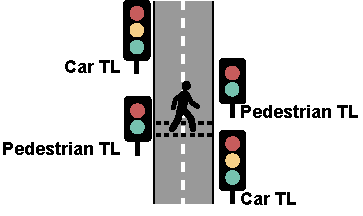
\includegraphics[width=0.5\textwidth]{images/running_example_schematic}
	\caption{Pedestrian crossing running example}
	\label{fig:overviewRunningExample}
\end{figure}

The behavior of the pedestrian TLs and car TLs are depicted as UML state machines \cite{objectmanagementgroupUnifiedModelingLanguage2017} in \autoref{fig:stateMachinesRunningExample}.

\begin{figure}[ht]
	\centering
	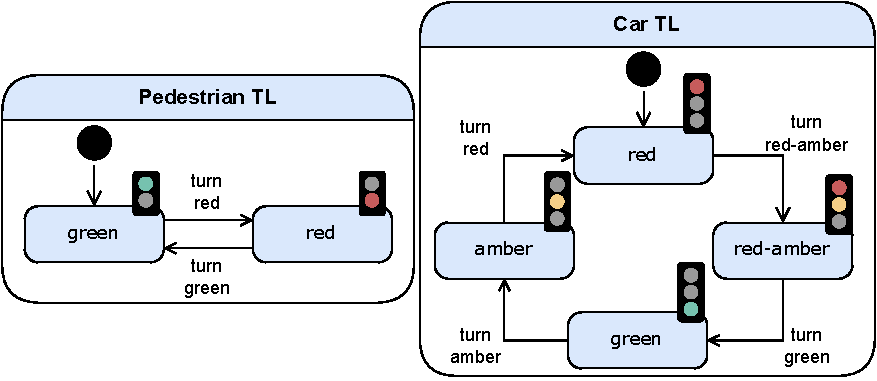
\includegraphics[width=1\textwidth]{images/running_example_models}
	\caption{Pedestrian TL and car TL as state machines}
	\label{fig:stateMachinesRunningExample}
\end{figure}

A \texttt{Pedestrian TL} can be \texttt{green} or \texttt{red}, while a \texttt{Car TL} has \texttt{red-amber} and \texttt{amber} as intermediate states between \texttt{red} and \texttt{green}.
How \textit{safe crossing} and \textit{progress in traffic} are achieved differs between the used coordination approaches.

The running example is deliberately kept simple because the focus should be on the coordination approaches, not the example's complexity.
Furthermore, the example does not need continuous variables and thus is insufficient to show Co-simulation's full capabilities compared to the other coordination approaches.
However, since continuous variables from physical systems cannot be represented in all coordination approaches, we opted for this running example, which represents a minimal denominator between all coordination approaches and is familiar to everyday life.

\section{Categories of coordination approaches} \label{sec:approaches}

\autoref{fig:overview} gives an overview of the different categories of coordination approaches.
The first two categories of coordination approaches mostly focus on the \textit{execution} level, i.e., they operate directly with source code or executable binaries.

\textbf{Co-simulation Tools} usually use the Functional Mock-up Interface (FMI)\footnote{\url{https://fmi-standard.org/}} standard, which defines executable systems parts, so-called Functional Mock-up Units (FMUs).
Each FMU consists of an executable and an XML model to describe its interface, for example, the FMU's exposed variables.
FMI is heavily used in the industry because it protects intellectual property (IP) since executables are black-box, i.e., do not expose implementation details.

\textbf{Coordination Languages} traditionally offer a shared tuple space for concurrent programs to read/write data from/to.
Separating \textit{coordination} from \textit{computation}, which seems natural today, was pioneered by coordination languages such as Linda \cite{carrieroLindaContext1989}.
% See if we can find a better citation for LF.
New coordination languages are being developed, such as Lingua Franca \cite{lohstrohReactorsDeterministicModel2020}, which use coordination mechanisms similar to ADLs but working with code on the execution level.

\begin{figure}[ht]
	\centering
	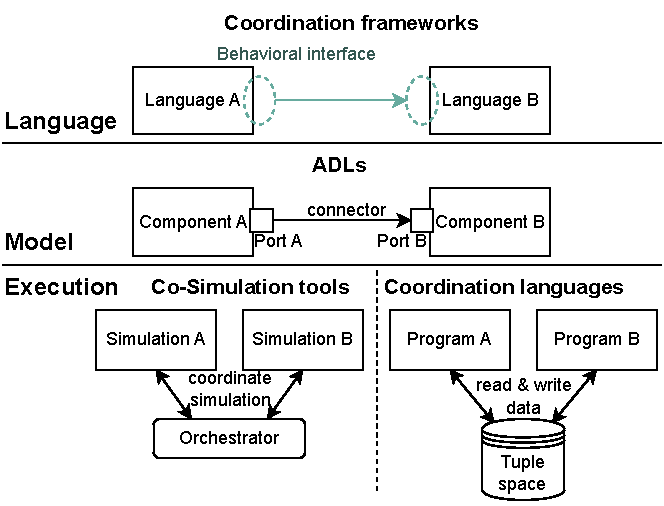
\includegraphics[width=0.75\textwidth]{images/overview}
	\caption{Overview of coordination approaches}
	\label{fig:overview}
\end{figure}

\textbf{Architecture Description Languages (ADLs)} operate on the \textit{model} level, i.e., each \textit{component} is given by a behavioral model, for example, a state machine.
Components coordinate through \textit{connectors} between them, resulting in an \textit{architectural configuration}.

\textbf{Coordination frameworks} allow the user to connect models conforming to \textit{different} behavioral languages using the concept of \textit{behavioral interfaces}.
In contrast, each ADL only allows one behavioral language, which must be used for each component.
Thus, they operate on the \textit{language} level and give modelers freedom to utilize different languages for varying aspects of the system.
In the following sections, we will describe each category in detail.

\subsection{Architecture description languages} \label{subsec:adl}
% General idea
Architecture Description Languages (ADLs) aim to describe the structure of systems, allowing developers to focus on high-level components and their connections rather than lines of source code~\cite{clementsSurveyArchitectureDescription1996,medvidovicClassificationComparisonFramework2000,medvidovicFrameworkClassifyingComparing1997}.
% What is an ADL, and what is not?
Many different ADLs have been proposed in the academic literature and by the industry~\cite{medvidovicClassificationComparisonFramework2000,woodsArchitectureDescriptionLanguages2005}.
Nevertheless, clearly defining ADLs is challenging due to overlap with general-purpose modeling languages~\cite{clementsSurveyArchitectureDescription1996}.

% Describing ADLs generally.
The three buildings blocks of ADLs are defined as (1) \textit{components}, (2) \textit{connectors}, (3) \textit{architectural configuration}~\cite{medvidovicClassificationComparisonFramework2000,medvidovicFrameworkClassifyingComparing1997}.
% Component
A \textit{component} is a unit of computation or data repository~\cite{medvidovicClassificationComparisonFramework2000}.
Components vary in size, ranging from representing individual services to entire systems.

% Connector
\textit{Connectors} serve as architectural elements to model interactions between components and the regulations that oversee those interactions~\cite{medvidovicClassificationComparisonFramework2000}.
A difference to components is that connectors must not be implemented as distinct entities such as message brokers but can also represent shared variables or links between applications realized by client-server protocols \cite{medvidovicClassificationComparisonFramework2000}.

% Architectural configuration
\textit{Architectural configuration}, also known as topology, represents the structural arrangement of components and connectors in a connected graph, defining the overall architecture~\cite{medvidovicClassificationComparisonFramework2000}.
This structure determines if the combined semantics results in the desired behavior.
For example, one can check for deadlocks and starvation.

% ADLS are formal and usually incorporate one formal language. Usually, a process algebra. They do not support multiple formal specification languages cite medvidovicClassificationComparisonFramework2000.
In addition, ADLs incorporate a formal language to enable analysis.
The first ADLs usually use process algebras such as Communicating Sequential Processes (CSP), Calculus of Communicating Systems (CCS), and $\pi$-calculus \cite{ozkayaAreWeThere2013}.
For example, Wright uses CSP \cite{allenFormalBasisArchitectural1997} while Darwin uses $\pi$-calculus \cite{mageeSpecifyingDistributedSoftware1995}.
More recent ADLs, such as MontiArc \cite{haberMontiArcArchitecturalModeling2014}, use automata to define the behavior of components.

However, no ADL supports multiple formal languages such as the coordination frameworks discussed in \autoref{subsec:frameworks} \cite{medvidovicClassificationComparisonFramework2000}.
Furthermore, despite the creation of numerous ADLs in the literature, they are not mainstream, i.e., used often by practitioners in the industry \cite{clementsSurveyArchitectureDescription1996,woodsArchitectureDescriptionLanguages2005,pandeyArchitecturalDescriptionLanguages2010,ozkayaAreWeThere2013,medvidovicMovingArchitecturalDescription2006}.

For this paper, we consider only ADLs that incorporate formal semantics and thus do not consider other modeling languages such as UML \cite{objectmanagementgroupUnifiedModelingLanguage2017} and ArchiMate \cite{theopengroupArchiMateSpecification2023} despite them being sometimes seen as ADLs and their usage in the industry.

A representative example of an ADL is given in  \autoref{lst:MontiArc-Crossing} showing the \textit{components} for the pedestrian crossing running example in MontiArc.

\lstinputlisting[
label=lst:MontiArc-Crossing,
language=MontiArc,
caption=MontiArc component for the pedestrian crossing]{listings/MontiArc-PedestrianCrossing.arc}

It defines three components: \textsf{PedestrianCrossing}, \textsf{PedestrianTL}, and \textsf{CarTL}.
Furthermore, the components \textsf{PedestrianTL} and \textsf{CarTL} define ports (line 10 and 15).
The \textit{architectural configuration} is defined in the \textsf{PedestrianCrossing} component (lines 1-7), which links the ports of the \textsf{PedestrianTL} and \textsf{CarTL} using a \textit{connector} (line 6).
% TODO: Add the full example in the artifacts (see pdf on overleaf)
The behavior of the \textsf{PedestrianTL} and \textsf{CarTL} components is omitted but given in \cite{timkrauterArtifactsCoordination2024}.

\subsection{Coordination languages}
% Define Coordination language and give examples
% Cite and survey
\cite{papadopoulosCoordinationModelsLanguages1998}

\subsection{Co-simulation tools}
% Define Co-simulation and give examples
\cite{gomesCoSimulationSurvey2019} % co-simulation survey

% Rewrite this part
Co-simulation aims to solve this challenge by composing the simulation of a system's parts into a global simulation \cite{gomesCoSimulationSurvey2019}.

For example, \cite{ekerTamingHeterogeneityPtolemy2003} propose an actor-oriented co-simulation approach, where each system part is represented as an actor.
An actor can communicate through its interfaces with other actors.
Their approach is implemented in the tool \textit{Ptolemy} and supports continuous time and state variables.
% FMI/FMU standard
Furthermore, the Functional Mock-up Interface (FMI)\footnote{\url{https://fmi-standard.org/}} is a co-simulation standard to exchange executable systems parts, so-called Functional Mock-up Units (FMUs).
Each FMU, similar to the actors in Ptolemy, comes with an XML model to describe its interface, for example, the FMU's exposed variables.
FMUs support continuous time and state variables and are widely used in the industry.

However, with co-simulations, one can only simulate systems, not check global behavioral properties.

\subsection{Coordination frameworks} \label{subsec:frameworks}
% Define Coordination-framework and give examples
% Surveys? Probably not.

% Distinguishing factors
The main differences between coordination frameworks and ADLs are as follows.

\textbf{(1) Heterogeneous models:} Coordination frameworks do not mandate one behavioral language or formalism for every model.
One can pick the most suitable language or formalism for each part of the system supported by the coordination framework.
For example, the car TL in the running example could be defined using a different behavioral language such as a UML activity diagram \cite{objectmanagementgroupUnifiedModelingLanguage2017}, a BPMN process model \cite{objectmanagementgroupBusinessProcessModel2013}, or a $\pi$-calculus term \cite{milnerCommunicatingMobileSystems2010}.

% Behavioral interfaces
\textbf{(2) Behavioral interfaces:} To coordinate between heterogeneous models \textit{behavioral interfaces} are used.
These interfaces are defined for each language or generally for all languages and represent a common understanding, which is needed when each language can be different.
Examples of coordination frameworks are Behavioral Coordination Operator Language (BCOoL) \cite{varalarsenBCOolBehavioralCoordination2016,varalarsenBehavioralCoordinationOperator2015} and BCoorLang \cite{krauterBehavioralConsistencyMultimodeling2023}.
% Ptolemy?

% BCoorLang is the new name. It's a bit close to BCOoL.
For example, using BCoorLang, one would define a \textit{system relationship model}, see \autoref{fig:exampleBCoorLang}, which defines existing behavioral models and their relations similar to the architectural configuration of ADLs.

\begin{figure}[ht]
	\centering
	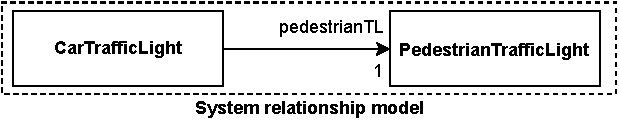
\includegraphics[width=0.7\textwidth]{images/running_example_BCorrLang}
	\caption{System relationship model for the running example}
	\label{fig:exampleBCoorLang}
\end{figure}

Using the behavioral relationship between \textsf{CarTrafficLight} and \textsf{PedestrianTrafficLight}, one can then define synchronizations of their behavior.
To describe the behavior of car TL and pedestrian TL, one can use the state machines defined in the running example (see \autoref{fig:stateMachinesRunningExample}) since the state machine behavioral language is supported in BCoorLang \cite{krauterBehavioralConsistencyMultimodeling2023}.


\section{Feature model} \label{sec:features}
The feature model aims to compare coordination approaches from different categories.
It cannot contain all the details from each approach since it must operate on a higher abstraction level to allow comparison across categories.
Thus, it can be too coarse-grained to compare approaches inside the same category.
For example, if one only wants to compare co-simulation approaches, the feature model might not distinguish them enough.
Consequently, one should use a taxonomy created only for co-simulation, such as \cite{gomesCoSimulationSurvey2019} instead.
However, our feature model still answers important questions.
For example, how can coordination be specified, and what is its semantics?
What are the goals of a coordination approach, how is the coordination implemented, and for which system domains is it suitable?

The feature model is shown in \autoref{fig:featureModelOverview}.
A coordination approach has three main features: \textit{Foundation}, \textit{Goal}, and \textit{Properties}.

\begin{figure}[ht]
	\centering
	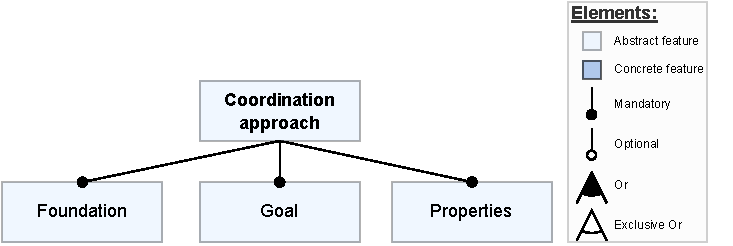
\includegraphics[width=0.85\textwidth]{images/root}
	\caption{Feature model overview}
	\label{fig:featureModelOverview}
\end{figure}

In the following sections, we will describe each abstract feature in detail.
% TODO: Add the full feature model as an artifact (at the end when the feature model is stable).
A complete diagram of the feature model is contained in \cite{timkrauterArtifactsCoordination2024}.

\subsection{Foundation}

\autoref{fig:foundationFeature} shows the \textbf {Foundation} feature, which consists of \textbf{Definition}, \textbf{Mechanism}, and \textbf{Semantics}.

% Maybe cut into two pieces. So, Definition and Semantics are not part of the same.
\begin{figure}[ht]
	\centering
	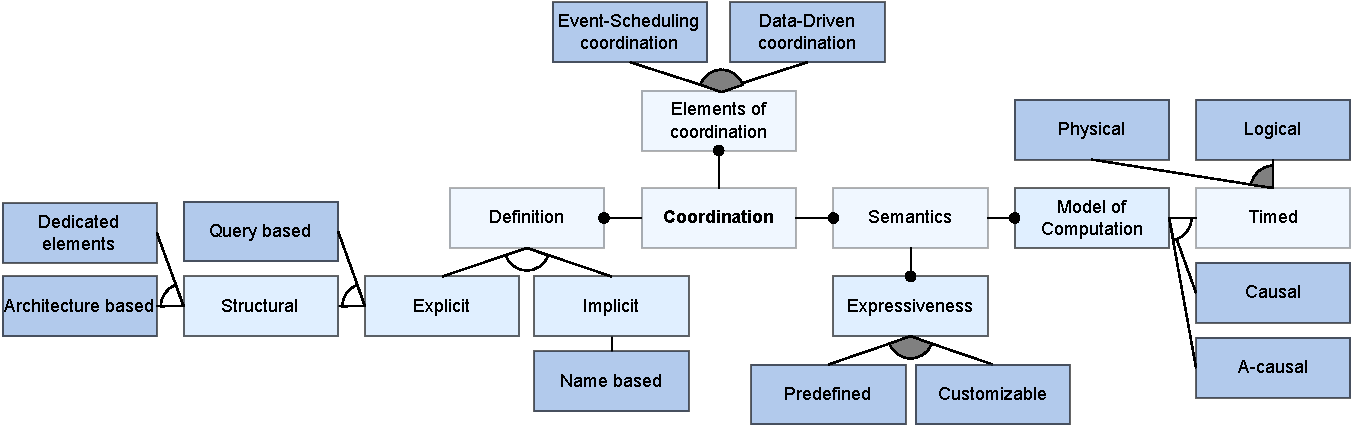
\includegraphics[width=1\textwidth]{images/coordination_feature}
	\caption{Foundation feature}
	\label{fig:foundationFeature}
\end{figure}

% TODO: Rewrite
\subsubsection{Definition} The definition of coordination can either be \textit{explicit} or \textit{implicit}.
An implicit definition is usually based on the names of model elements.
For example, one could synchronize transitions of state machines if they have identical names.

Explicit definition is either \textit{query based} or \textit{structural}.
% Query-based example
For example, in BCOoL \cite{varalarsenBCOolBehavioralCoordination2016,varalarsenBehavioralCoordinationOperator2015}, one can write expressions to define which elements should coordinate.

A structural definition of coordination uses \textit{dedicated elements} or is \textit{architecture based}.
For example, interactions in BCoorLang are specified by dedicated elements, while coordination in ADLs depends on the architectural configuration \cite{medvidovicClassificationComparisonFramework2000}, i.e., how ports of components are connected.

\subsubsection{Mechanism} The main mechanism driving coordination can be \textit{event scheduling}, \textit{data exchange}, or a mix of both.
Sometimes this is also called \textit{control-driven} and \textit{data-driven} \cite{papadopoulosCoordinationModelsLanguages1998,varalarsenBCOolBehavioralCoordination2016}.
Typically, a coordination approach is focused on one of the two mechanisms, but both can be supported.

First, \textit{event scheduling} synchronizes or mandates a specific order for events, i.e., state changes in different components.
Usually, event scheduling is used when components are given by behavioral models since there might not be a clear concept of an event in a programming language.
For example, in BCOoL \cite{varalarsenBehavioralCoordinationOperator2015}, one can define relationships between events, such as happens before or synchronizes.

\textit{Data-exchange} means components communicate by exchanging data.
For example, in Co-simulation \cite{gomesCoSimulationSurvey2019}, components send data from output to input ports, or exposed variables of multiple components are coupled such that they should be the same. % Causal vs. A-causal MoC
However, data exchange might also happen between components during the synchronization of events, which is why both coordination mechanisms can be supported simultaneously.

% TODO: Rewrite
\subsubsection{Semantics} The semantics feature consists of \textit{expressiveness} and \textit{model of computation}.
The expressiveness of coordination can be \textit{predefined}, i.e., a user has a fixed set of coordination mechanisms or \textit{customizable}.
For example, in BCOoL, the user can employ the Clock Constraints Specification Language (CCSL) \cite{andreSyntaxSemanticsClock2009} when defining coordination \cite{varalarsenBCOolBehavioralCoordination2016,varalarsenBehavioralCoordinationOperator2015}.

Coordination approaches utilize different \textit{models of computation} (MoC).
% What is a model of computation? Where does the terminology come from?
% causal a-causal also identified as causality in gomesCoSimulationSurvey2019
We define three MoCs: \textit{timed}, \textit{causal}, \textit{a-causal}, where \textit{timed} is either \textit{physical} or \textit{logical}.
% We should define that event and state-changing elements mean the same, i.e., any observable action in a model/component.
% Causal (events and data)
% TODO: Rewrite this. It is more about data
The causal MoC means that the coordination approach can define \textit{causal} relationships between events of different components.
For example, a transition in a state machine raises an event that causes a reaction in an activity diagram due to the defined coordination.
% A-causal
A-causal MoC is employed in Co-simulation, which can deal with sets of differential equations.
For example, a variable in one equation should equal a variable in a different equation.
One variable does not cause the other to change.
Instead, they should be equal at any time.

% Timed::Logical
\textit{Logical} time means that coordination approaches define when events/state changes happen.
Typically, one defines that events take place simultaneously or that one event causes another event or causes another event with a fixed delay.
For example, a delay could be 50 milliseconds of logical time, corresponding to time in a simulation that can run arbitrarily fast. 
% Timed::Physical --> other term wall-clock time see gomesCoSimulationSurvey2019 and its citations
In contrast, \textit{physical} time describes time passing in the physical world.
One can, for example, define that one event should happen 50 milliseconds after another.
In Lingua Franca \cite{lohstrohReactorsDeterministicModel2020}, logical time "chases" physical time, i.e., logical time tries to match the physical time provided by the execution platform.
% Logical time, however, always lags behind physical time.


\subsection{Goal} % Or even call it motivation
We identified three different \textit{goals} of coordination approaches: \textbf{simulation}, \textbf{execution}, and \textbf{formal verification}, see \autoref{fig:goalFeature}.
Usually, approaches focus on one goal.
For example, co-simulation tools provide a simulation, while others, such as coordination frameworks, might provide formal verification in addition to simulation.
However, which types of dynamic systems can be simulated varies and is discussed in the next section.

\begin{figure}[ht]
	\centering
	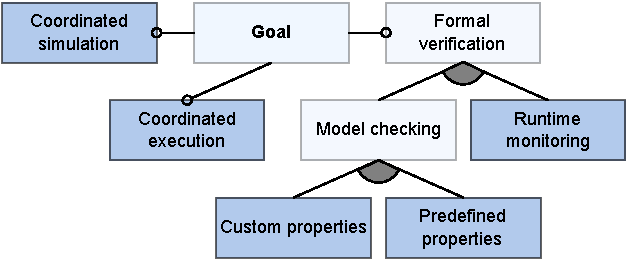
\includegraphics[width=0.7\textwidth]{images/goal_feature}
	\caption{Goal feature}
	\label{fig:goalFeature}
\end{figure}

\subsubsection{Simulation} The most common goal of coordination approaches is a coordinated simulation of multiple components or behavioral models representing the entire system.
A coordinated simulation is useful because the composition of multiple components can lead to unexpected behavior, often called \textit{emergent behavior} \cite{ekerTamingHeterogeneityPtolemy2003}.
Emergent behavior can be dealt with early in development before implementing each component and its interactions.
Co-simulation tools such as DACCOSIM \cite{galtierFMIBasedDistributedMultisimulation2015} or MECSYCO \cite{camusCosimulationCyberphysicalSystems2018} are examples of approaches that have coordinated simulation as their goal.
Simulation is also implemented by coordination frameworks such as BCoorLang \cite{krauterBehavioralConsistencyMultimodeling2023} and BCOol \cite{varalarsenBehavioralCoordinationOperator2015}.
Even recent ADLs such as MontiArc \cite{haberMontiArcArchitecturalModeling2014} provide simulation capabilities.

\subsubsection{Execution} In contrast to coordinated simulation, which often only aims to find errors during development, the goal of coordination approaches such as coordination languages is a coordinated execution after system deployment.

For example, the coordination language Linda aims to provide virtual shared memory as an alternative to message-passing \cite{carrieroLindaAlternativeMessagepassing1994}, which is a widely spread communication model to implement decoupled communication, i.e., coordination of software systems.

Furthermore, the recently developed polyglot coordination language \textit{Lingua Franca} provides determinism guarantees during distributed execution \cite{lohstrohLinguaFrancaDeterministic2021}.
Thus, it aims to provide a better coordination framework for concurrent \textit{execution}.


\subsubsection{Formal verification} Another goal of coordination approaches, especially for safety-critical systems, is formal verification.
Formal verification can be used before the system is deployed (\textit{model checking}) or while it is running (\textit{runtime monitoring}).

We encountered coordination approaches that check \textit{predefined properties}, while others support \textit{custom properties}.
% (Definition 5)
For example, the ADL Wright \cite{allenFormalBasisArchitectural1997} can check \textit{deadlock freedom} of component interactions.
% Darwin and we are checking custom properties: mageeBehaviourAnalysisSoftware1999 krauterBehavioralConsistencyMultimodeling2023
The coordination framework for behavioral consistency \cite{krauterBehavioralConsistencyMultimodeling2023} supports custom properties written in temporal logic such as Linear Temporal Logic (LTL) and Computational Tree Logic (CTL).
We are unaware of approaches supporting runtime monitoring, but it is the next logical step when applying formal verification techniques throughout the development lifecycle.

\subsection{Properties}
% Categorization corresponds to the different co-simulation approaches described in gomesCoSimulationSurvey2019.
We identified several common \textit{properties} when analyzing coordination approaches, see \autoref{fig:propertiesFeature}.
We will now explain each property in detail.

\begin{figure}[ht]
	\centering
	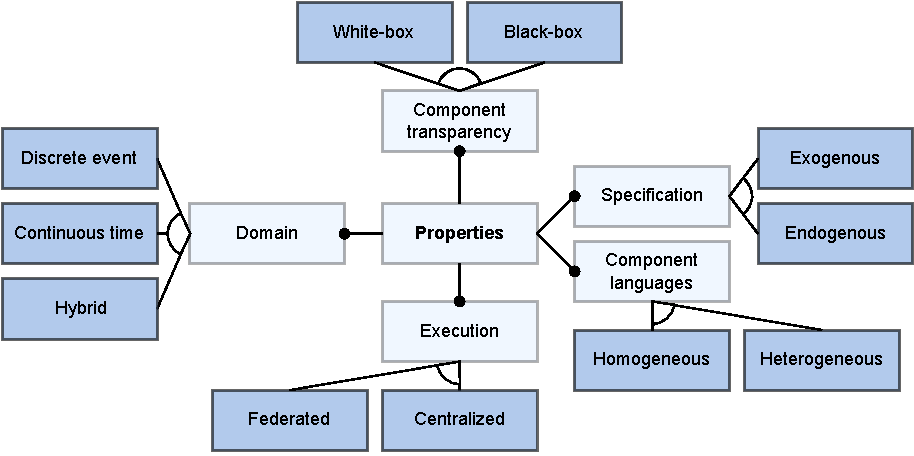
\includegraphics[width=1\textwidth]{images/properties_feature}
	\caption{Properties feature}
	\label{fig:propertiesFeature}
\end{figure}

% Maybe add some examples and descriptions here.
\subsubsection{Domain} Coordination approaches operate in different domains, similar to the categorization of co-simulation approaches in \cite{gomesCoSimulationSurvey2019}.
First, if a coordination approach is part of the \textit{Discrete event} domain, means it assumes discrete state changes.
Typically, coordination frameworks and ADLs operate in this domain since variables change their values discontinuously during execution.

Second, coordination approaches in the \textit{continuous time} domain support components to have a state that evolves continuously over time.
Often, components are given by sets of differential equations, which omit continuous variable changes, such as physical systems involving springs and dampeners, see \cite{gomesCoSimulationSurvey2019}.

Third, the \textit{hybrid} domain is a mix of the first two domains that occur in the co-simulation of cyber-physical systems.
Concretely, components should coordinate where the state of some components changes discretely while the state of other components evolves continuously in time.
Two strategies deal with hybrid systems: one either adapts the components from the continuous time to the discrete event domain or vice versa \cite{gomesCoSimulationSurvey2019}.

The choice of a coordination approach depends on the nature of the system at hand.
For instance, software systems can usually be modeled in the discrete event domain, while physical or cyber-physical systems operate in the continuous time or even hybrid domain.

\subsubsection{Specification} We distinguish between \textit{intrusive} and \textit{non-intrusive specification} of coordination.
For example, when using the coordination language Linda \cite{carrieroLindaContext1989}, one uses basic operations such as \textsf{out} and \textsf{in} inside components to create and read tuples in the shared tuple space, i.e., shared memory.
Thus, Linda is \textit{intrusive} since one has to add coordination operations to the components.

On the other hand, \textit{non-intrusive} coordination approaches do not require changes to the components.
However, components must be created with coordination in mind to expose possible coordination points.
For example, BCOol \cite{varalarsenBehavioralCoordinationOperator2015} uses behavioral interfaces to define events, which can then be used to specify \textit{non-intrusive} coordination rules outside the components.

In a nutshell, some approaches allow changing coordination without touching the components, which is impossible in others.
This is exactly the difference between non-intrusive and intrusive coordination specifications.

\subsubsection{Component languages} Coordination approaches typically only support \textit{homogeneous} components.
For example, coordination languages, such as Lingua Franca \cite{lohstrohReactorsDeterministicModel2020}, typically only support coordination if each component is given in the same programming language.

Similarly, most ADLs only coordinate components defined using the same modeling language.
As stated earlier, ADLs often use a specific process algebra to define the behavior of its components.
However, coordination frameworks allow \textit{heterogeneous} components, i.e., components specified in different behavioral modeling languages.
For example, BCoorLang \cite{krauterBehavioralConsistencyMultimodeling2023} supports all modeling languages where one can clearly define \textit{state structure} and which \textit{elements can change state} during execution.

\subsubsection{Implementation} Coordination approaches are generally implemented differently.
First, in a \textit{co-simulation}, each component runs as an independent black box.
Then, a coordination approach provides an \textit{orchestrator} which controls the passage of time and moves output data from one component to another \cite{gomesCoSimulationSurvey2019}, i.e., facilitates coordination.

An alternative is a \textit{unified execution} where components are white box and executed together.
Coordination languages often mandate the same underlying \textit{programming language} for each component to provide coordination, while coordination frameworks rely on a \textit{formal language} for a coordinated execution.

For example, the coordination language Lingua Franca \cite{lohstrohReactorsDeterministicModel2020} provides infrastructure written in a given programming language for a unified execution.
A distributed, i.e., federated execution is in the early stages of development for Lingua Franca but not officially supported\footnote{\url{https://www.lf-lang.org/docs/writing-reactors/distributed-execution}} yet, which is why we did not consider it for our feature model.
The coordination framework BCoorLang \cite{krauterBehavioralConsistencyMultimodeling2023} uses graph or term-rewriting as formal languages to coordinate heterogeneous components.


\section{Application of the feature model} \label{sec:application}
\autoref{tab:classification} shows the application of our feature model to four different coordination approaches.
Each approach represents a co-simulation tool (\textit{DACCOSIM}), coordination language (\textit{Linda} \cite{carrieroLindaContext1989,carrieroLindaAlternativeMessagepassing1994}), ADL (\textit{MontiArc} \cite{haberMontiArcArchitecturalModeling2014}), or coordination framework (\textit{BCoorLang} \cite{krauterBehavioralConsistencyHeterogeneous2021,krauterBehavioralConsistencyMultimodeling2023}).
% TODO: Why did we choose these? Representative feature sets? Recent publications? --> Not Linda
However, we classified 16 approaches, including the four chosen representatives.
All classifications are available in the artifacts of this paper \cite{timkrauterArtifactsCoordination2024}.

% Could even have two tables for better sizing and add 1-2 approaches.
% TODO: Double-check DACCOSIM and ensure it is the best co-simulation pick.
\begin{table}
	\centering
	\caption{Approach classification}
	\label{tab:classification}
	\resizebox{\textwidth}{!}{
	\SetTblrInner{colsep=2pt}
	\begin{tblr}{
			column{2-Z} = {c},
			hline{1, 2, Z} = {-}{1.2pt, solid}, % Z is the last row/column
			hline{7, 11} = {-}{dashed},
			vline{2-Y} = {2-Z}{solid},
		}
		\diagbox[linewidth=1.1pt,font=\bfseries]{Feature}{Approach} & \textbf{DACCOSIM} & \textbf{Linda} & \textbf{MontiArc} & \textbf{BCoorLang} \\
		
		\textbf{Coordination} \\
		\hspace{2mm} Definition & Name based & Name based & Architecture based & Dedicated elements \\
		\hspace{2mm} Mechanism & Data-Exchange & Data-Exchange & Data-Exchange & Event-Scheduling \\ % everything ends in coordination here in the feature model
		\hspace{2mm} Expressiveness & Predefined & Predefined & Predefined & Predefined \\
		\hspace{2mm} MoC & A-causal, Causal & Causal & Timed:Logical, Causal & Timed:Logical \\
		
		\textbf{Goal} \\
		\hspace{2mm} Simulation & + & - & + & + \\
		\hspace{2mm} Execution & - & + & - & - \\
		\hspace{2mm} Formal verification & - & - & - & Custom properties \\
		
		\textbf{Properties} \\
		\hspace{2mm} Domain & Hybrid & Discrete event & Discrete event & Discrete event \\
		\hspace{2mm} Specification & Intrusive & Intrusive & Intrusive & Non-Intrusive \\
		\hspace{2mm} Component languages & Homogeneous & Homogeneous & Homogeneous & Heterogeneous \\	
		\hspace{2mm} Implementation & Co-simulation & PL & PL & Formal language \\
	\end{tblr}
	}
\end{table}

We compare BCoorLang, MontiArc, and Linda in \autoref{fig:venn-Linda}.
The figure shows a Venn diagram comparing the feature sets of each approach, where the numbers in each colored part state the number of features contained.

\begin{figure}[ht]
	\centering
	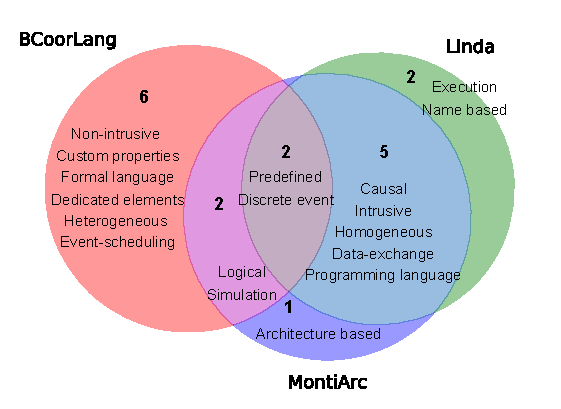
\includegraphics[width=0.5\textwidth]{images/venn_linda}
	\caption{Feature comparison: BCoorLang, MontiArc, and Linda}
	\label{fig:venn-Linda}
\end{figure}

For example, the one at the bottom of \autoref{fig:venn-Linda} describes that MontiArc has one \textit{unique} feature (\textsf{Definition:Architecture based}), while the two in the middle declares that all three approaches share two \textit{common} features (\textsf{Expressiveness:Predefined, Domain:Discrete event}), see \autoref{tab:classification}.
All classification data and scripts to generate diagrams such as \autoref{fig:venn-Linda} are included in \cite{timkrauterArtifactsCoordination2024}.

From \autoref{fig:venn-Linda}, one can see that most Linda features overlap with either BCoorLang or MontiArc.
Only \textsf{Execution} as a goal and \textsf{Definition:Name based} for coordination are not shared.
This makes sense since Linda and other initial coordination languages have greatly influenced the development of ADLs and coordination frameworks, which happened afterward.
Furthermore, one can see that coordination frameworks, i.e., BCoorLang (the diagram is similar for BCOol \cite{varalarsenBehavioralCoordinationOperator2015,varalarsenBCOolBehavioralCoordination2016}) greatly differ from ADLs and coordination languages.
Multiple unique features, such as heterogeneous component languages and an underlying implementation in a formal language that permit formal verification exist,


Similarly, \autoref{fig:venn-DACCOSIM} compares the features of BCoorLang and MontiArc with the co-simulation tool DACCOSIM.
One can see that BCoorLang and DACCOSIM do not have many features in common, probably due to their different goals as a coordination approach.
Co-simulation approaches like DACCOSIM have unique features such as an A-causal MoC and a hybrid domain.

% TODO: Change color of DACCOSIM to not be the same as Linda in the previous fig.
\begin{figure}[ht]
	\centering
	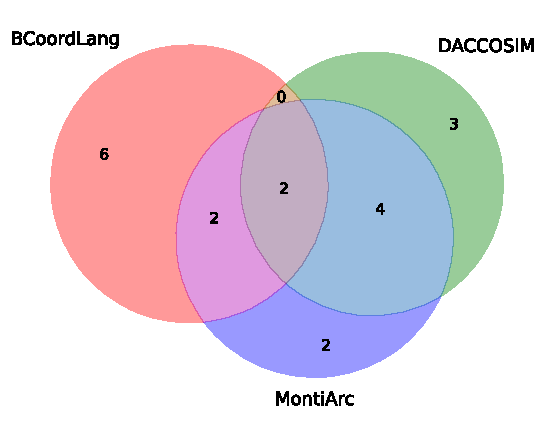
\includegraphics[width=0.5\textwidth]{images/venn_daccosim}
	\caption{Feature comparison: BCoorLang, MontiArc, and DACCOSIM}
	\label{fig:venn-DACCOSIM}
\end{figure}


\section{Findings} \label{sec:findings}
 % Interprete the previous classification
% Typical features (clusters) for ADLs, Coordination language, Co-simulation, and coordination frameworks.
% Maybe they can somehow be visualized nicely using some clusters with overlaps (Venn diagrams, Upset plots?)


% Commonalities between clusters

% Differences between clusters

% What are the unique features of each approach? Does this match their intended usage scenarios?

% ADLs, coordination languages, and coordination frameworks usually apply to software systems, while co-simulation applies to hybrid systems, i.e., cyber-physical systems. Thus, they support different MoCs and domains and have different goals.

\textbf{Coordination frameworks do not support Data-Exchange:} All coordination frameworks we have encountered support \textsf{Event-Scheduling} but not \textsf{Data-Exchange} as a coordination mechanism.
This is likely because data exchange is difficult to achieve when heterogeneous components are allowed.
However, data exchange is omnipotent in real-world systems, so it is the main coordination mechanism used in co-simulation tools and coordination languages.
Thus, for coordination frameworks to be employed in real-world scenarios, they must support data exchange.
Furthermore, it is identified as important future work in \cite{krauterBehavioralConsistencyMultimodeling2023,varalarsenBCOolBehavioralCoordination2016}.

\section{Conclusion \& future work} \label{sec:conclusion}

\bibliographystyle{splncs04}
\bibliography{bib}

\end{document}
